\documentclass[10pt]{article}

%------------------------------------------------------
%   PACKAGES
%------------------------------------------------------

% Default 
\usepackage{graphicx}
\usepackage[backend=biber,style=numeric,sorting=ynt]{biblatex}

% Additional
\usepackage{amsmath}
\usepackage{textcomp, gensymb}
\usepackage{placeins}
\usepackage{tabularray} 
\usepackage{xcolor}
\usepackage{placeins}

\addbibresource{references.bib}

\title{Prism Spectrometer} 
\author{Rahmanyaz Annyyev, Hikmat Gulaliyev} 
\date{02 March 2024} 

\begin{document}

\maketitle

\begin{abstract}
In this experiment, we utilize a prism spectrometer---an optical device that separates light into its constituent frequencies---to measure the refractive index of a prism. A collimator with a slit is used to produce a parallel beam of light emitted by a mercury lamp, which is then passed through the prism. The light is then refracted and dispersed into its constituent frequencies. The angle of deviation of the light is measured and used to calculate the refractive index of the prism using a special relation. A graph of the index of refraction versus wavelength and the inverse square of the wavelength is plotted, and the constants of the Cauchy equation are obtained. The results are in line with the theoretical values, and the experiment is successful.
\end{abstract}

\section{Introduction}

The visible spectrum is the portion of electromagnetic radiation that is visible to the human eye. It is composed of light with wavelengths between 380 and 780 nm. Each wavelength, or frequency of light is perceived as a different color by the human eye \cite{Marcus_1998}. Spectrum analysis is the study of measure and interpretation of electromagnetic spectra. It is used in various fields such as physics, chemistry, and astronomy. One of the most important tools in spectrum analysis is the prism spectrometer. 

A prism spectrometer is an optical device, and it is composed of a collimator, a prism, and a telescope. The collimator is a device that produces a parallel beam of light. It is composed of an adjustable slit on one end and a converging lens on the other. The slit is used to control the width of the entering light, and the lens is used to focus the light into a parallel beam. As the beam exits the collimator, it impinges on the prism. The prism rests on a rotatable table, and it is used to refract and disperse the light into its constituent colors. The telescope is used to observe the dispersed light, and it is composed of a lens and an eyepiece. The set of parallel beams of different wavelengths form images of the slit. The telescope can be rotated with the aid of the reticle to position the images for each spectral line. 
The instrument that is used throughout the experiment to measure the angles is called a vernier scale. Note that a mercury lamp was used as a source of light.

The experiment is divided into two parts. Before proceeding, we follow two preliminary steps. First, we adjust the telescope on a distant object to ensure that it is properly focused. Next, we calibrate the collimator to ensure that the light is parallel.

In the first part, we measure the apex angle of the prism---the angle between the two faces of the prism. The prism is placed on the table such that the angle is towards the collimator. Next, we rotate the telescope and find two positions where the light is \textit{reflected} from the prism. The image of the slit is observed through the telescope, and the telescope is further adjusted until the image falls on the reticle. The positions are then read from the vernier scale. The apex angle is given by the relation
\begin{equation}
    \alpha = \frac{\texttt{Position1} + \texttt{Position2}}{2},
\end{equation}
where $\texttt{Position}_1$ and $\texttt{Position}_2$ are the two angles. Several measurements are taken, and the average is calculated using the formula
\begin{equation}
    \bar{\alpha} = \frac{1}{N} \sum_{i=1}^{N} \alpha_i,
\end{equation}
where $N$ is the number of measurements.

In the second part, we use the spectrometer to measure the refractive index of the prism. It is a measure of how much the light is bent as it passes through the prism. Examine Figure~\ref{fig:1}. As you can see, $\delta$ is the angle of deviation of the light---the angle between the incident and emergent beams of light, and $\alpha$ is the angle of the prism. To find the refractive index of the prism, we measure the \textit{minimum} deviation angle of the light. 

\begin{figure}[ht]
    \centering
    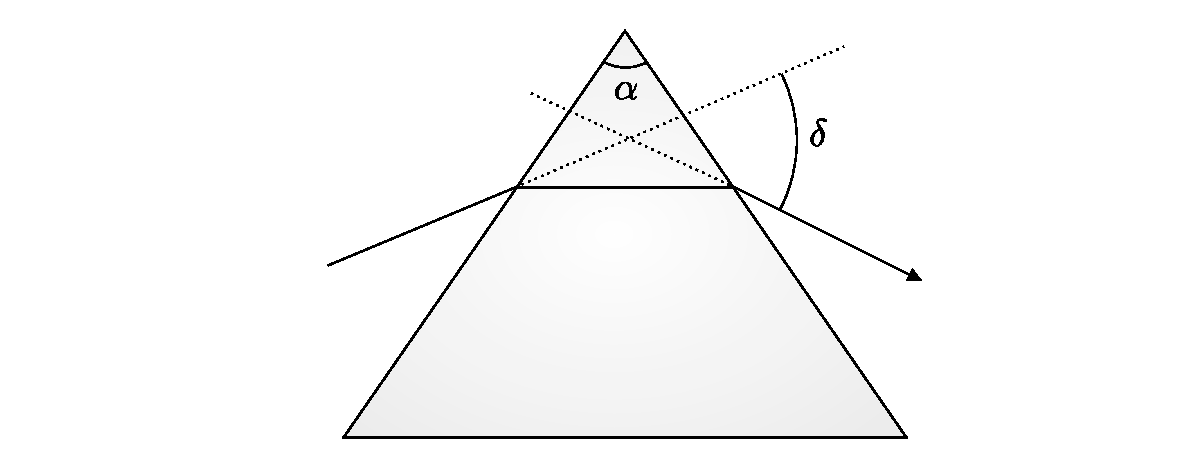
\includegraphics[scale=0.6]{figures/f1.pdf}
    \caption{Refraction of light through a prism.}
    \label{fig:1}
\end{figure}

The minimum angle of deviation occurs when the angle of incidence is equal to the angle of emergence. Hence, in this case, the refractive index of the prism is given by the relation
\begin{equation}
    \label{eq:1}
    n = \frac{\sin\left((\delta_{min}+\alpha) / 2 \right)}{\sin\left(\alpha / 2\right)},
\end{equation}
which is derived from Snell's law,
\begin{equation}
    n_1 \sin(\theta_1) = n_2 \sin(\theta_2),
\end{equation}
where $n_1$ and $n_2$ are the refractive indices of the two media, and $\theta_1$ and $\theta_2$ are the angles of incidence and refraction, respectively. The methodology for finding the minimum deviation angle is as follows. We need to determine two positions. First, we remove the prism from the table and record the position of the telescope such that it is parallel to the collimator and the image of the slit is adjusted to fall on the reticle. This is the first position. Next, we place the prism back on the table such that one of the faces makes an angle of $45\degree$ with the beam coming from the collimator. Next, we rotate the telescope and find the position where the light is \textit{refracted} from the prism. The spectral lines in several colors are observed through the telescope, and the latter is further adjusted until \textit{each} line falls on the reticle. Then, the telescope is rotated further until a point where the direction of movement of the spectral lines reverses in direction. This is the second position. The deviation angle is given by the relation
\begin{equation}
    \delta_{min} = 360\degree - \texttt{Position1} + \texttt{Position2}.
\end{equation}

A dispersion curve is a graph of the refractive index versus wavelength. It can be represented using the Cauchy equation,
\begin{equation}
    n(\lambda) = A + \frac{B}{\lambda^2} + \frac{C}{\lambda^4} + \cdots,
\end{equation}
where $A$, $B$, and $C$ are constant pertaining to a specific material. The dispersion curve is used to determine the refractive index of a material at a specific wavelength.

\section{Data \& Results}

The results of the first part of the experiment are shown in Table~\ref{tab:1}. The average angle of the prism is given by $\bar{\alpha} = 59.87\degree$.
\begin{table}[ht]
    \label{tab:1}
    \centering
    \vspace{4mm}

    \begin{tblr}{
        cells = {halign = c, valign = m},
        row{odd} = {bg = lightgray!5},
        row{1} = {bg = lightgray!20},
        hlines = {},
        vlines = {},
        cell{5}{1}={c=2}{l}
    }
        Position \#1 & Position \#2 & $\alpha_i$ \\
        $52\degree 46'$ & $293\degree 01'$ & $59.86\degree$ \\
        $52\degree 52'$ & $293\degree 05'$ & $59.88\degree$ \\
        $52\degree 48'$ & $293\degree 03'$ & $59.86\degree$ \\
        & & $\bar{\alpha} = 59.87\degree$ \\
    \end{tblr}
    \caption{Data for the prism angle, $\alpha$.}
\end{table}

The results of the second part of the experiment are shown in Table~\ref{tab:2}. The wavelengths of the spectral lines were taken from the table given in the laboratory manual. 
\begin{table}[ht]
    \label{tab:2}
    \centering
    \vspace{4mm}

    \begin{tblr}{
        cells = {halign = c, valign = m},
        row{odd} = {bg = lightgray!5},
        row{1} = {bg = lightgray!20},
        hlines = {},
        vlines = {}
    }
        $\lambda$ (nm), Color & Position \#1 & Position \#2 & $\delta_{min}$ & $n$ \\
        $404.6$, Violet & $351\degree 48'$ & $27\degree 40'$ & $40.19$ & $1.536$ \\
        $435.8$, Blue & $351\degree 48'$ & $28\degree 41'$ & $39.18$ & $1.524$ \\
        $546.1$, Green & $351\degree 48'$ & $29\degree 28'$ & $38.31$ & $1.514$ \\
        $579.1$, Orange & $351\degree 48'$ & $29\degree 49'$ & $38.02$ & $1.511$ \\
    \end{tblr}
    \caption{Data for the refractive index versus wavelength.}
\end{table}
After evaluating the refractive index for each wavelength, we proceeded to plot two graphs. The first graph shows the relationship between the refractive index of the prism and the wavelength of the light. The second graph shows the relationship between the refractive index and the inverse square of the wavelength, and the line is the least squares fit of the data. The values of the constants $A$ and $B$ are obtained and shown in the graph. The results are shown in Figures~\ref{fig:2} and \ref{fig:3}.

\begin{figure}[ht]
    \centering
    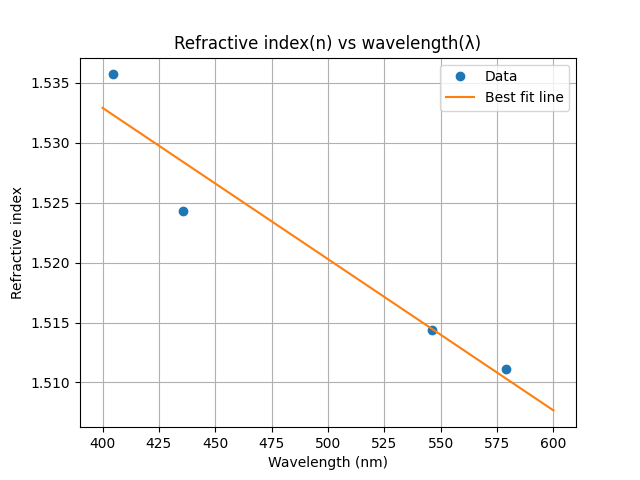
\includegraphics[scale=0.7]{figures/f2.png}
    \caption{Refraction index versus wavelength.}
    \label{fig:2}
\end{figure}

\begin{figure}[ht]
    \centering
    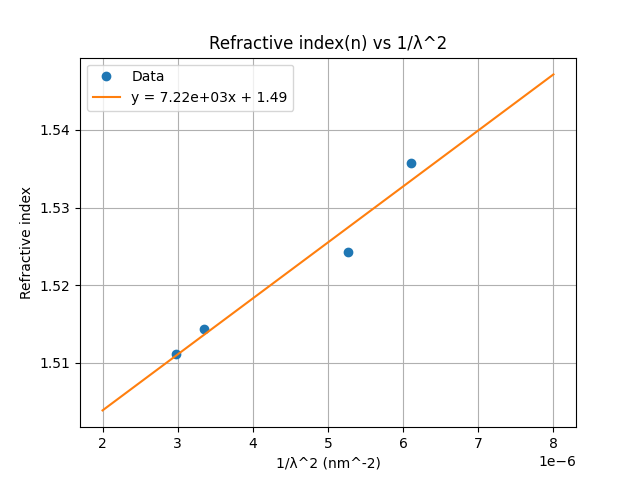
\includegraphics[scale=0.7]{figures/f3.png}
    \caption{Refraction index versus inverse square of wavelength.}
    \label{fig:3}
\end{figure}

\FloatBarrier % Prevents figures from floating into the next section
 
\section{Discussion \& Conclusion}


Due to the analog nature of this experiment, human error is inevitable. In particular, manually reading the angles using a vernier scale introduces some error. Moreover, manually adjusting the telescope to find the minimum deviation angle is another source of error.

Before and during the experiment, some assumptions were made, such as the light source is monochromatic, the prism is perfectly shaped and uniform, the refractive index of air is 1, and the telescope is perfectly calibrated. These assumptions may not hold true in real life and may introduce some error to the results.

Despite these limitations, the experiment is in line with the theoretical values. Everything, except for the number of spectral lines, aligns with the theory. This discrepancy might be explained by the fact that some of these lines are too close together for the human eye to distinguish.

In conclusion, the experiment was successful, with results largely in line with the theoretical values. Introducing optoelectronics in further studies could minimize human error and improve the accuracy of the results.
\printbibliography

\end{document}